\documentclass{../../slides-style}

\slidetitle{Контейнеры и генерики}{18.04.2025}

\begin{document}

    \begin{frame}[plain]
        \titlepage
    \end{frame}

    \section{Контейнеры}

    \begin{frame}
        \frametitle{Интерфейсы контейнеров}
        \begin{columns}
            \begin{column}{0.65\textwidth}
                \begin{itemize}
                    \item IEnumerable --- штука, из которой можно последовательно получать элементы
                    \item ICloneable --- штука, от которой можно делать глубокую копию
                    \item ICollection --- абстрактная коллекция
                    \item IDictionary --- расширение ICollection, абстрактный словарь
                    \item IList --- расширение ICollection, коллекция, к элементам которой можно обращаться по индексу
                \end{itemize}
            \end{column}
            \begin{column}{0.3\textwidth}
                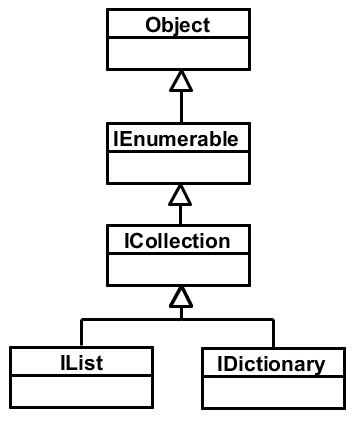
\includegraphics[width=\textwidth]{interfaces.png}
            \end{column}
        \end{columns}
    \end{frame}

    \begin{frame}[fragile]
        \frametitle{Энумератор}
        \begin{itemize}
            \item Абстрагирует обход коллекции, не может её модифицировать
            \begin{itemize}
                \item Обобщённая позиция внутри коллекции
                \item Как правило, требует доступа к внутренним полям коллекции
            \end{itemize}
            \item Реализует интерфейс IEnumerator
            \begin{itemize}
                \item Свойство Current
                \begin{itemize}
                    \item Изначально --- перед первым элементом
                \end{itemize}
                \item MoveNext()
                \begin{itemize}
                    \item Возвращает false после последнего элемента
                \end{itemize}
                \item Reset()
                \begin{itemize}
                    \item Можно не реализовывать, тогда кидает NotSupportedException
                \end{itemize}
            \end{itemize}
            \item Компилятор знает про IEnumerable:
            \begin{minted}{csharp}
foreach (var i in list) { 
    Console.Write(i); 
}
            \end{minted}
            \item Инвалидируется при изменении коллекции (но Current продолжает работать)
        \end{itemize}
    \end{frame}

    \begin{frame}
        \frametitle{Негенериковые коллекции}
        \begin{itemize}
            \item ArrayList, реализует IList, ICollection, IEnumerable, ICloneable
            \item BitArray,  реализует ICollection, IEnumerable, ICloneable
            \item Hashtable, реализует IDictionary, ICollection, IEnumerable, ICloneable
            \item Queue, реализует ICollection, IEnumerable, ICloneable
            \item SortedList, реализует IDictionary, ICollection, IEnumerable, ICloneable
            \item Stack, реализует ICollection, IEnumerable, ICloneable
        \end{itemize}
    \end{frame}

    \begin{frame}[fragile]
        \frametitle{Почему негенериковые коллекции --- плохо}
        \begin{itemize}
            \item boxing/unboxing
            \begin{itemize}
                \item \mintinline{csharp}|list.Add(1);|
            \end{itemize}
            \item Типобезопасность
            \begin{itemize}
                \item \mintinline{csharp}|list.Add(1);|
                \item \mintinline{csharp}|list.Add("hello");|
            \end{itemize}
            \item Понижающие касты
            \begin{itemize}
                \item \mintinline{csharp}|var str = list[1] as string;|
            \end{itemize}
            \item Поэтому придумали генерики:
            \begin{minted}{csharp}
var list = new List<string>();
list.Add("hello");
var str = list[0];
            \end{minted}
            \begin{itemize}
                \item Так обычно пишут в книгах <<C\# для суперпрофессионалов>>, но это не совсем правда...
            \end{itemize}
        \end{itemize}
    \end{frame}

    \section{Параметрический полиморфизм}

    \begin{frame}
        \frametitle{Типизация}
        \begin{itemize}
            \item Данные --- это просто строки битов
            \item Пример --- теория множеств
            \begin{itemize}
                \item \{\} --- 1
                \item \{\{\}\} --- 2
                \item Парадокс Рассела
                \begin{itemize}
                    \item \enquote{Пусть А --- множество всех множеств, которые не содержат себя в качестве своего элемента. Содержит ли А само себя в качестве элемента?}
                \end{itemize}
                \item Типы ограничивают допустимые операции над значениями
                \item Виды типизации
                \begin{itemize}
                    \item Динамическая или статическая
                    \item Сильная или слабая
                \end{itemize}
            \end{itemize}
        \end{itemize}
    \end{frame}

    \begin{frame}[fragile]
        \frametitle{Ad-hoc полиморфизм}
        \begin{itemize}
            \item Перегрузка
            \item Приведение
        \end{itemize}
        Пример:
        \begin{minted}{csharp}
1 + 1.0
        \end{minted}

        \begin{itemize}
            \item \mintinline{csharp}|"+" (int + int, int + float, float + int, float + float)|
            \item \mintinline{csharp}|"+" (int + int, float + float)|
            \item \mintinline{csharp}|"+" (float + float)|
        \end{itemize}
    \end{frame}

    \begin{frame}
        \frametitle{Универсальный полиморфизм}
        \begin{itemize}
            \item Полиморфизм подтипов (сабтайпинг, наследование)
            \begin{itemize}
                \item 1..10 --- подынтервал 1..100, следовательно, подтип
                \item Принцип подстановки Лисков
            \end{itemize}
            \item Параметрический полиморфизм
            \begin{itemize}
                \item \mintinline{fsharp}|id: x: 'T -> x: 'T|
                \item \mintinline{fsharp}|id<int>(2)|
                \item \mintinline{fsharp}|id<string>("Cthulhu fhtagn!")|
                \item \mintinline{fsharp}|List<'T>| --- набор параметрически полиморфных функций
            \end{itemize}
        \end{itemize}
    \end{frame}

    \begin{frame}
        \frametitle{Типы}
        \begin{itemize}
            \item Элементарные типы
            \item Конструкторы типов
            \begin{itemize}
                \item Подъязык для описания сложных типов
            \end{itemize}
            \item Структурное равенство и равенство по имени
            \item Выражения над типами
            \begin{itemize}
                \item Генерик --- это функция, принимающая набор параметров-типов и возвращающая тип
            \end{itemize}
        \end{itemize}

        Подробности: Cardelli, Luca, and Peter Wegner. "On understanding types, data abstraction, and polymorphism." ACM Computing Surveys (CSUR) 17.4 (1985): pp. 471-523.
    \end{frame}

    \section{Генерики в .NET}

    \begin{frame}[fragile]
        \frametitle{Генерики в .NET}
        \begin{itemize}
            \item System.Collections.Generic
            \begin{minted}{csharp}
List<string> listOfStrings = new();
            \end{minted}
            \item Не требуют исходного кода генерика
            \begin{itemize}
                \item Информация о параметрах-типах есть в байт-коде
            \end{itemize}
            \item Не выполняют boxing, если параметр-тип --- тип-значение
            \begin{itemize}
                \item Для каждого параметра типа-значения при инстанциировании порождается новый код (как в C++)
                \item Для каждого параметра ссылочного типа байт-код переиспользуется (как в Java)
                \begin{itemize}
                    \item Но не происходит стирание
                \end{itemize}
            \end{itemize}
        \end{itemize}

        Генерик-методы:
        \begin{minted}{csharp}
nt[] myInts = {1, 5, 2, 8, 4};
Array.Sort<int>(myInts);
        \end{minted}
    \end{frame}

    \begin{frame}[fragile]
        \frametitle{Выражения инициализации}
        \begin{minted}{csharp}
int[] myArrayOfInts = { 0, 1, 2, 3, 4, 5, 6, 7, 8, 9 };

var myGenericList = new List<int> { 0, 1, 2, 3, 4, 5, 6, 7, 8, 9 };

var myList = new ArrayList { 0, 1, 2, 3, 4, 5, 6, 7, 8, 9 };
        \end{minted}
    \end{frame}

    \begin{frame}[fragile]
        \frametitle{Свои генерик-методы}
        \begin{minted}{csharp}
static void Swap(ref int a, ref int b)
{
    int temp = a;
    a = b;
    b = temp;
}
        \end{minted}
        \hspace{2cm} $\Downarrow$
        \begin{minted}{csharp}
static void Swap<T>(ref T a, ref T b)
{
   T temp = a;
   a = b;
   b = temp;
}
        \end{minted}
    \end{frame}

    \begin{frame}[fragile]
        \frametitle{Использование}
        \begin{minted}{csharp}
int a = 10, b = 90;
Swap<int>(ref a, ref b);

string s1 = "Hello", s2 = "There";
Swap<string>(ref s1, ref s2);

bool b1 = true, b2 = false;
Swap(ref b1, ref b2);
        \end{minted}
    \end{frame}

    \begin{frame}[fragile]
        \frametitle{Генерик-классы}
        \begin{scriptsize}
            \begin{minted}{csharp}
public class Point<T>
{
   private T xPos;
   private T yPos;

   public Point(T xVal, T yVal) {
       xPos = xVal;
       yPos = yVal;
   }
   
   public T X {
       get { return xPos; }
       set { xPos = value; }
   }

   public override string ToString() => $"[{xPos}, {yPos}]";

   public void ResetPoint() {
       xPos = default(T);
       yPos = default(T);
   }
}
            \end{minted}
        \end{scriptsize}
    \end{frame}

    \begin{frame}[fragile]
        \frametitle{Использование}
        \begin{minted}{csharp}
Point<int> p = new(10, 10);
Point<double> p2 = new(5.4, 3.3);

var p = new Point<int>(10, 10);
var p2 = new Point<double>(5.4, 3.3);
        \end{minted}
    \end{frame}

    \begin{frame}
        \frametitle{Рекомендации по именованию}
        \begin{itemize}
            \item Параметр тип должен называться \textbf{T} или хотя бы начинаться с \textbf{T}
            \begin{itemize}
                \item Например, \mintinline{csharp}|Data<TKey, TValue>|
            \end{itemize}
            \item Если генерики отличаются только параметрами-типами и находятся в разных файлах, то:
            \begin{itemize}
                \item Можно добавлять число параметров-типов в имя файла через ``\textbf{`}''
                \begin{itemize}
                    \item Например, Data`1.cs, Data`2.cs
                \end{itemize}
                \item Можно параметры-типы включать в имена файлов в фигурных скобках
                \begin{itemize}
                    \item Например, Data\{T\}.cs, Data\{TKey,TValue\}.cs
                \end{itemize}
            \end{itemize}
        \end{itemize}
    \end{frame}

    \begin{frame}[fragile]
        \frametitle{Открытые и закрытые типы}
        \framesubtitle{Как оно устроено внутри}
        \begin{itemize}
            \item \textbf{Открытый тип} --- тип с неспецифицированными параметрами-типами, создание его экземпляров невозможно
            \item \textbf{Закрытый тип} --- тип, у которого для всех параметров-типов указаны фактические типы
        \end{itemize}
        \begin{scriptsize}
            \begin{minted}{csharp}
internal sealed class DictionaryStringKey<TValue> 
        : Dictionary<String, TValue> {
}

public static class Program {
    public static void Main() {
        // Открытый тип
        Type t = typeof(Dictionary<,>);
        // Открытый тип
        t = typeof(DictionaryStringKey<>);
        // Закрытый тип
        t = typeof(DictionaryStringKey<Guid>);
    }
}
            \end{minted}
        \end{scriptsize}
    \end{frame}

    \begin{frame}[fragile]
        \frametitle{Статические конструкторы}
        Каждый закрытый тип имеет \textbf{свой} объект-тип, статический конструктор вызовется для каждого параметра-типа
        \vspace{0.8cm}
        \begin{footnotesize}
            \begin{minted}{csharp}
internal sealed class GenericTypeThatRequiresAnEnum<T> {
    static GenericTypeThatRequiresAnEnum() {
        if (!typeof(T).IsEnum) {
            throw new ArgumentException("T must be an enumerated type");
        }
    }
}
            \end{minted}
        \end{footnotesize}
        \vspace{0.8cm}
        Обычно так делать не надо, есть ограничения
    \end{frame}

    \begin{frame}[fragile]
        \frametitle{Способ прострелить себе ногу}
        \framesubtitle{\textcopyright\, Андрей Акиньшин}
        \begin{small}
            \begin{minted}{csharp}
class Foo<T>
{
    public static int Bar;
}

void Main()
{
    Foo<int>.Bar++;
    Console.WriteLine(Foo<double>.Bar);
}
            \end{minted}
        \end{small}
        Вообще, мутабельные static-поля в generic-классах не нужны. Ещё более вообще, мутабельные static-поля не нужны.
    \end{frame}

    \begin{frame}[fragile]
        \frametitle{Идентичность типов-генериков}
        Иногда вместо
        \begin{footnotesize}
            \begin{minted}{csharp}
List<DateTime> dtl = new();
            \end{minted}
        \end{footnotesize}
        пишут
        \begin{footnotesize}
            \begin{minted}{csharp}
internal sealed class DateTimeList : List<DateTime> { }
...
DateTimeList dtl = new();
            \end{minted}
        \end{footnotesize}
        \vspace{5mm}
        Теряется эквивалентность типов:
        \begin{footnotesize}
            \begin{minted}{csharp}
Boolean sameType = (typeof(List<DateTime>) == typeof(DateTimeList));
            \end{minted}
        \end{footnotesize}
        \vspace{5mm}
        Можно
        \begin{footnotesize}
            \begin{minted}{csharp}
using DateTimeList = System.Collections.Generic.List<System.DateTime>;
            \end{minted}
        \end{footnotesize}
    \end{frame}

    \begin{frame}[fragile]
        \frametitle{Генерики и вложенные классы}
        Вложенные в генерик классы могут использовать его параметры-типы (и сами считаются генериками)
        \vspace{5mm}
        \begin{footnotesize}
            \begin{minted}{csharp}
public class Outermost<T>
{
    public class Inner<U>
    {
        public class Innermost1<V> {}
        public class Innermost2 {}
    }
}
            \end{minted}
        \end{footnotesize}
        \vspace{5mm}
        Объект вложенного класса нельзя создать, не указав параметры-типы объемлющего класса
    \end{frame}

    \section{Ограничения}
    
    \begin{frame}[fragile]
        \frametitle{Ограничения}
        \begin{minted}{csharp}
public class MyGenericClass<T> where T : new()
public class MyGenericClass<T> where T : new(), class
public class MyGenericClass<T, U> 
    where T : new() 
    where U: class
        \end{minted}

        Доступные ограничения:
        \begin{itemize}
            \item \mintinline{csharp}|where T : struct|
            \item \mintinline{csharp}|where T : class|
            \item \mintinline{csharp}|where T : new()|
            \item \mintinline{csharp}|where T : NameOfBaseClass|
            \item \mintinline{csharp}|where T : NameOfInterface|
        \end{itemize}
    \end{frame}

    \begin{frame}[fragile]
        \frametitle{Пример 1}
        \framesubtitle{Primary constraint}
        \begin{footnotesize}
            \begin{minted}{csharp}
internal sealed class PrimaryConstraintOfStream<T> where T : Stream 
{
    public void M(T stream) 
        => stream.Close();
}
            \end{minted}
        \end{footnotesize}
    \end{frame}

    \begin{frame}[fragile]
        \frametitle{Пример 2}
        \framesubtitle{Primary constraint}
        \begin{footnotesize}
            \begin{minted}{csharp}
internal sealed class PrimaryConstraintOfClass<T> where T : class {
    public void M() 
    {
        // Поскольку T - ссылочный тип, присвоить ему null допустимо
        T temp = null;
    }
}
            \end{minted}
        \end{footnotesize}
    \end{frame}

    \begin{frame}[fragile]
        \frametitle{Пример 3}
        \framesubtitle{Secondary constraint}
        \begin{footnotesize}
            \begin{minted}{csharp}
private static List<TBase> ConvertIList<T, TBase>(IList<T> list)
        where T : TBase 
{
    List<TBase> baseList = new(list.Count);
    for (int index = 0; index < list.Count; index++) 
    {
        baseList.Add(list[index]);
    }
    return baseList;
}
            \end{minted}
        \end{footnotesize}
    \end{frame}

    \begin{frame}[fragile]
        \frametitle{Пример 4}
        \framesubtitle{Constructor constraint}
        \begin{footnotesize}
            \begin{minted}{csharp}
internal sealed class ConstructorConstraint<T> where T : new() {
    public static T Factory() {
        // Тут подойдут любые типы-значения и 
        // ссылочные типы с public-конструктором без параметров
        return new T();
    }
}
            \end{minted}
        \end{footnotesize}
    \end{frame}

    \begin{frame}[fragile]
        \frametitle{Генерики и сравнения}
        Так работает:
        \begin{footnotesize}
            \begin{minted}{csharp}
private static void ComparingAGenericTypeVariableWithNull<T>(T obj) {
    if (obj == null) { /* Никогда не вызовется для типов-значений */ }
}
            \end{minted}
        \end{footnotesize}
        \vspace{5mm}
        А так нет:
        \begin{footnotesize}
            \begin{minted}{csharp}
private static void ComparingTwoGenericTypeVariables<T>(T o1, T o2) {
    if (o1 == o2) { }
}
            \end{minted}
        \end{footnotesize}
    \end{frame}

    \section{Вариантность}

    \begin{frame}[fragile]
        \frametitle{Вариантность}
        \begin{minted}{csharp}
public void f(Tuple<object, object> x)
{
    ...
}

f(new Tuple<object, object>(apple1, apple2));
f(new Tuple<Apple, Apple>(apple1, apple2));  // Ошибка компиляции
        \end{minted}
        \vspace{3mm}
        Чтобы нельзя было делать так:
        \begin{minted}{csharp}
public void f(Tuple<object, object> x)
{
    x.Item1 = new Battleship();
}
        \end{minted}
    \end{frame}

        \begin{frame}[fragile]
        \frametitle{Виды вариантности}
        \begin{footnotesize}
            \begin{itemize}
                \item \textbf{Ковариантность} --- A $\leq$ B => G<A> $\leq$ G<B>
                \begin{minted}{csharp}
void PrintAnimals(IEnumerable<Animal> animals) {
    for (var animal in animals)
        Console.WriteLine(animal.Name);
}
                \end{minted}
                --- IEnumerable<любой наследник Animal> тоже ок, IEnumerable ковариантен
                \item \textbf{Контравариантность} --- A $\leq$ B => G<B> $\leq$ G<A>
                \begin{minted}{csharp}
void CompareCats(IComparer<Cat> comparer) {
    var cat1 = new Cat("Otto");
    var cat2 = new Cat("Troublemaker");
    if (comparer.Compare(cat2, cat1) > 0) 
        Console.WriteLine("Troublemaker wins!");
}
                \end{minted}
                --- IComparer<любой предок Cat> тоже ок, IComparer контравариантен
                \item \textbf{Инвариантность} --- A $\leq$ B => G<A> и G<B> никак не связаны
                \begin{itemize}
                    \item Пример с Tuple выше
                \end{itemize}
            \end{itemize}
        \end{footnotesize}
    \end{frame}

    \begin{frame}[fragile]
        \frametitle{Ковариантность массивов}
        \begin{minted}{csharp}
string[] a = new string[1];
object[] b = a;
b[0] = 1;
        \end{minted}
        --- System.ArrayTypeMismatchException, ошибка времени выполнения!
    \end{frame}

    \begin{frame}[fragile]
        \frametitle{Вариантность функциональных типов}
        \framesubtitle{Контравариантность по типам аргументов}
        \begin{minted}{csharp}
public class A
{
    public static void f(Func<string, object> a)
    {
        a("1");
    }
}
...
Func<object, object> b = x => x.ToString();
A.f(b);
        \end{minted}
    \end{frame}

    \begin{frame}[fragile]
        \frametitle{Вариантность функциональных типов}
        \framesubtitle{Ковариантность по возвращаемому значению}
        \begin{minted}{csharp}
Func<Object, ArgumentException> fn1 = null;
Func<Object, Exception> fn2 = fn1;
        \end{minted}

        Обратите внимание, ref-параметры сразу делают функцию инвариантной
    \end{frame}

    \begin{frame}[fragile]
        \frametitle{Явное указание вариантности для интерфейсов}
        \begin{minted}{csharp}
public interface IContainer<out T>
{
   T GetItem();
}


public interface IContainer<out T>
{
   void SetItem(T item);  // ошибка компиляции
   T GetItem();
}
        \end{minted}
    \end{frame}

    \begin{frame}
        \frametitle{Как это можно себе представлять}
        \begin{center}
            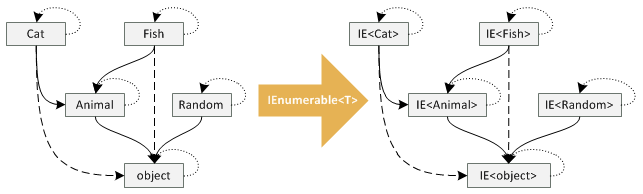
\includegraphics[width=0.6\textwidth]{covariantFunctors.png}

            \vspace{4mm}
            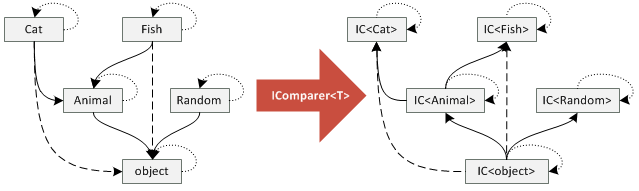
\includegraphics[width=0.6\textwidth]{contravariantFunctors.png}
        \end{center}
            
        \url{http://tomasp.net/blog/variance-explained.aspx/}
    \end{frame}

\end{document}
